\section{Gradient Descent}


\begin{definition}{Gradient Descent}\\
Gradient Descent is an optimization algorithm for finding the minimum of a function by iteratively moving in the direction of steepest descent. For a cost function $J(\theta)$, the update rule is:
\[\theta_j = \theta_j - \alpha \frac{\partial}{\partial\theta_j}J(\theta) \quad \forall j = 0,...n\]
where $\alpha$ is the learning rate.
\end{definition}

\begin{concept}{Why Gradient Descent?}\\
The explicit solution for linear regression using the normal equation doesn't work well for large datasets because:
\begin{itemize}
    \item Matrix operations have approximately cubic runtime complexity
    \item Normal equation becomes too time-consuming for more than 20,000 features or samples
    \item The normal equation might become numerically unstable if features are highly correlated
\end{itemize}
In these cases, gradient descent provides a more efficient approach.
\end{concept}

\begin{KR}{Implementing Gradient Descent for Linear Regression}
\paragraph{Initialize parameters}
Start with random values for parameters $\theta_0, \theta_1, ..., \theta_n$

\paragraph{Repeat until convergence}
For each parameter $\theta_j$, update it simultaneously:
\[\theta_j = \theta_j - \alpha \frac{1}{M}\sum_{m=1}^{M}(h_\theta(x^{(m)}) - y^{(m)})x^{(m)}_j\]
where:
\begin{itemize}
    \item $h_\theta(x^{(m)})$ is the current prediction for input $x^{(m)}$
    \item $y^{(m)}$ is the expected output
    \item $x^{(m)}_j$ is the $j$-th feature of the $m$-th training example (with $x^{(m)}_0 = 1$)
\end{itemize}

\paragraph{Key considerations}
\begin{itemize}
    \item Parameters must be updated simultaneously, not sequentially
    \item The learning rate $\alpha$ controls the step size
    \item A large learning rate might cause divergence
    \item A small learning rate leads to slow convergence
\end{itemize}
\end{KR}

\begin{example}{Gradient Descent Step-by-Step}
Consider a simple linear regression with two data points: (1,1) and (2,2).
\begin{itemize}
    \item Start with parameters $\theta_0 = 0, \theta_1 = 0$
    \item Initial prediction: $\hat{y} = 0 + 0 \times x = 0$
    \item Error for first point: $1 - 0 = 1$
    \item Error for second point: $2 - 0 = 2$
    \item With learning rate $\alpha = 0.1$, after first iteration:
    \begin{itemize}
        \item $\theta_0 = 0 - 0.1 \times \frac{1}{2} \times (1 + 2) = 0 - 0.15 = -0.15$
        \item $\theta_1 = 0 - 0.1 \times \frac{1}{2} \times (1 \times 1 + 2 \times 2) = 0 - 0.25 = -0.25$
    \end{itemize}
    \item After several iterations, parameters converge to $\theta_0 = 0, \theta_1 = 1$
\end{itemize}
\end{example}

\subsection{Types of Gradient Descent}

\begin{definition}{Batch Gradient Descent}\\
Batch gradient descent uses all training examples in each iteration. For each parameter $\theta_j$:
\[\theta_j = \theta_j - \alpha \frac{1}{M}\sum_{m=1}^{M}(h_\theta(x^{(m)}) - y^{(m)})x^{(m)}_j\]
Advantages:
\begin{itemize}
    \item Computes the true gradient of the cost function
    \item More stable convergence
\end{itemize}
Disadvantages:
\begin{itemize}
    \item Slow for very large datasets
    \item Requires all data to be in memory
\end{itemize}
\end{definition}

\begin{definition}{Stochastic Gradient Descent (SGD)}\\
Stochastic gradient descent updates parameters using only one randomly selected training example in each iteration:
\[\theta_j = \theta_j - \alpha (h_\theta(x^{(m)}) - y^{(m)})x^{(m)}_j\]
Advantages:
\begin{itemize}
    \item Much faster for large datasets
    \item Can process data online (one example at a time)
\end{itemize}
Disadvantages:
\begin{itemize}
    \item More erratic updates and convergence
    \item May require more iterations
\end{itemize}
\end{definition}

\begin{definition}{Mini-Batch Gradient Descent}\\
Mini-batch gradient descent is a compromise that updates parameters using a small batch of training examples (typically 10-1000) in each iteration:
\[\theta_j = \theta_j - \alpha \frac{1}{b}\sum_{m \in B}(h_\theta(x^{(m)}) - y^{(m)})x^{(m)}_j\]
where $B$ is the mini-batch and $b$ is its size.
Advantages:
\begin{itemize}
    \item More efficient than batch gradient descent
    \item More stable than stochastic gradient descent
    \item Can leverage vectorized operations
\end{itemize}
\end{definition}

\raggedcolumns
\columnbreak

\subsection{Learning Rate Optimization}

\begin{definition}{Learning Rate}
The learning rate $\alpha$ in gradient descent controls the step size at each iteration. It affects convergence:
\begin{itemize}
    \item Too small: algorithm converges very slowly
    \item Too large: algorithm might overshoot the minimum and diverge
\end{itemize}
\end{definition}

\begin{concept}{Learning Rate Optimization}
Several strategies can improve learning rate effectiveness:
\begin{itemize}
    \item \textbf{Decay Rate}: Start with a larger learning rate and reduce it over time using $\alpha_t = \frac{1}{1+decay\_rate \times t}\alpha_0$
    \item \textbf{Adaptive Methods}: Use algorithms like Adam or Adagrad that adjust learning rates based on the behavior of gradients
\end{itemize}
\end{concept}

\mult{2}

\begin{KR}{Choosing the Right Learning Rate}
\paragraph{Start with a sensible default}
Begin with a moderate learning rate \\(e.g., 0.01 or 0.001)

\paragraph{Learning rate search}
\begin{itemize}
    \item Try a range of learning rates \\(e.g., 1.0, 0.1, 0.01, 0.001, 0.0001)
    \item Plot the learning curves (cost vs. iterations)
    \item Too high: cost increases or oscillates wildly
    \item Too low: cost decreases very slowly
    \item Just right: cost decreases steadily and quickly
\end{itemize}

\paragraph{Adaptive learning rates}
Consider using adaptive optimization algorithms:
\begin{itemize}
    \item Adam: Adaptive Moment Estimation
    \item RMSprop: Root Mean Square Propagation
    \item Adagrad: Adaptive Gradient Algorithm
\end{itemize}

\paragraph{Learning rate schedules}
Implement learning rate decay:
\begin{itemize}
    \item Step decay: Reduce by a factor after fixed number of epochs
    \item Exponential decay: $\alpha_t = \alpha_0 \times e^{-kt}$
    \item 1/t decay: $\alpha_t = \alpha_0 / (1 + kt)$
\end{itemize}
\end{KR}

\begin{example2}{Learning Rate Impact}
Consider training a linear regression model with different learning rates:
\begin{itemize}
    \item Cost function:\\ $J(\theta) = \frac{1}{2M}\sum_{m=1}^{M}(y^{(m)} - \theta^T x^{(m)})^2$
    \item Initial parameters: $\theta = [0, 0]^T$
    \item 100 training examples with true parameters \\$\theta^* = [2, 3]^T$
\end{itemize}
\tcblower
With learning rate $\alpha = 0.01$:
\begin{itemize}
    \item Iteration 1: $J(\theta) = 6.5$
    \item Iteration 10: $J(\theta) = 2.1$
    \item Iteration 100: $J(\theta) = 0.2$
    \item Final parameters: $\theta \approx [1.9, 2.8]^T$ (close to true values)
\end{itemize}

With learning rate $\alpha = 1.0$:
\begin{itemize}
    \item Iteration 1: $J(\theta) = 20.3$ (increasing!)
    \item Iteration 10: $J(\theta) = 156.7$ (diverging)
    \item Algorithm fails to converge
\end{itemize}

With learning rate $\alpha = 0.0001$:
\begin{itemize}
    \item Iteration 1: $J(\theta) = 6.49$
    \item Iteration 10: $J(\theta) = 6.2$
    \item Iteration 100: $J(\theta) = 4.8$
    \item Very slow convergence
\end{itemize}
\end{example2}

\multend

\begin{concept}{Convergence Criteria}
Common stopping criteria for gradient descent:
\begin{itemize}
    \item \textbf{Maximum iterations}: Stop after a fixed number of iterations
    \item \textbf{Cost threshold}: Stop when the cost is below a threshold
    \item \textbf{Small gradient}: Stop when the gradient magnitude is below a threshold
    \item \textbf{Parameter change}: Stop when parameters change very little between iterations
    \item \textbf{Validation performance}: Stop when performance on validation set stops improving
\end{itemize}
\end{concept}

\raggedcolumns
\columnbreak

\subsubsection{Gradient Descent for Linear Regression}

\begin{KR}{Gradient Descent for Linear Regression}\\
Adjust the slope with rotation and the y-intercept with translation.

\paragraph{Step 1}
Start with a random line (e.g., $y = 2x + 3$)

\paragraph{Step 2}
Pick a large number of repetitions $R$

\paragraph{Step 3}
Pick a small number for the learning rate $LR$

\paragraph{Step 4}
Pick a random point (repeat $R$ times):
\begin{itemize}
    \item \textbf{Slope}: Add $LR \cdot (x - x_{new}) \cdot (y - y_{new})$
    \item \textbf{Intercept}: Add $LR \cdot (y - y_{new})$
\end{itemize}
\end{KR}

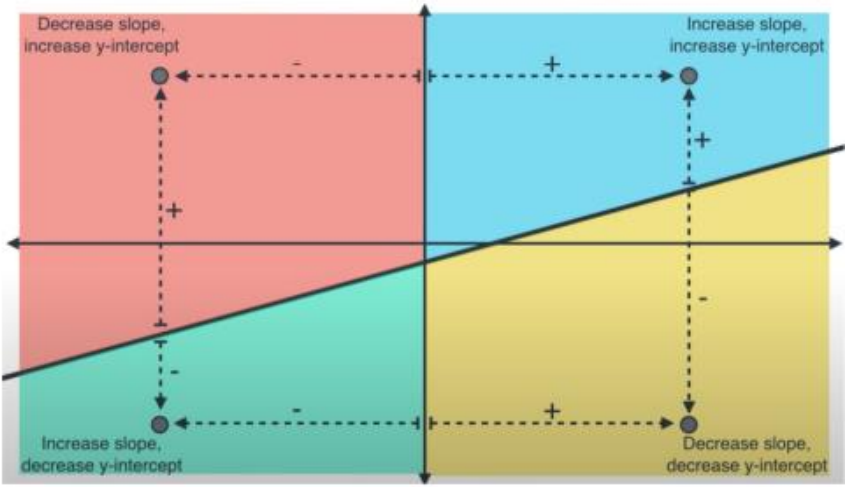
\includegraphics[width=\linewidth]{gradient_descent.png}